\chapter{GSM}

\section{Overview}

GSM (Global System for Mobile Communications, originally Groupe Sp\'ecial Mobile), is a very popular standard that describes protocols for second generation (2G) digital cellular networks used by mobile phones. GSM networks usually operate in the 900 MHz, 1800 MHz or 1900 MHz bands. It supports a full data rate of 9.6 kbits/sec or 14.4 kbits/sec using better codecs.


\section{System Architecture}

A GSM Public Land Mobile Network (PLMN) consists of at least one Service Area managed by a Mobile Switching Center (MSC) connected to the Public Switched Telephone Network  (PSTN).

\begin{figure}
\centering
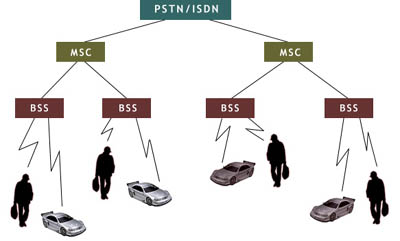
\includegraphics[scale=0.7]{archPLMN}
\caption[GSM PLMN architecture]{The architecture of a GSM Public Land Mobile Network (PLMN).
\emph{Source: \url{http://wireless.arcada.fi/MOBWI/material/CN\_1\_2.html}}}
\end{figure}

The network structure can be divided into the following discrete sections:
\begin{itemize}
\item Base Station Subsystem
\item Network and Switching Subsystem
\item Operation Subsystem
\end{itemize}


\subsection{Base Station Subsystem (BSS)}

A base station subsystem consists of
\begin{itemize} 
\item a Base Station Controller (BSC) and
\item at least one Base Transceiver Station (BTS) for Mobile Stations (MS). A mobile station can be a cell phone, or any electronic equipment such as a Personal Digital Assistant (PDA) with a phone interface.
\end{itemize}

The area served by a single BTS is considered a Network Cell. One or more BTSs are managed by a single BSC.  A group of BSSs can be managed as a Location Area (Location Area) provided all those BSSs are being managed by the same MSC.


\begin{figure}
\centering
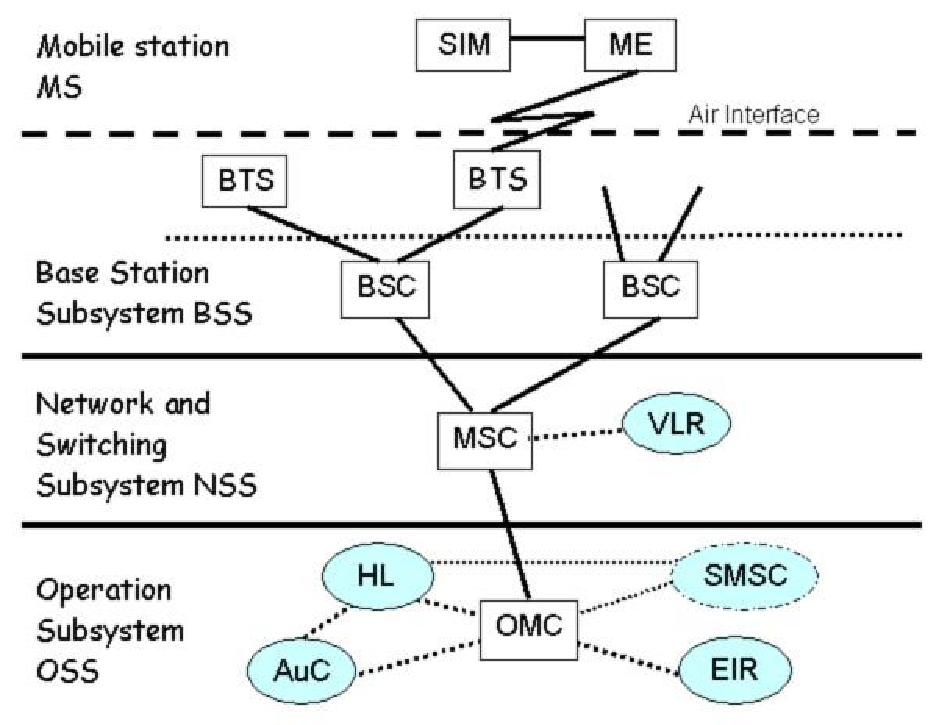
\includegraphics[scale=0.7]{archMSCServiceArea}
\caption[Network architecture for a single MSC Service Area]{The GSM network architecture for a single MSC controlled Service Area.
\emph{Source: \url{http://wireless.arcada.fi/MOBWI/material/CN\_1\_2.html}}}
\end{figure}


An MSC may also be connected via a Gateway MSC (GMSC) to other MSCs or the Public Switched Telephone Network (PSTN) with the Integrated Services Digital Network (ISDN) option. The Inter-Working Function (IWF) of a GMSC makes it possible to connect the circuit switched data paths of a GSM network with the PSTN/ISDN.

\begin{figure}
\centering
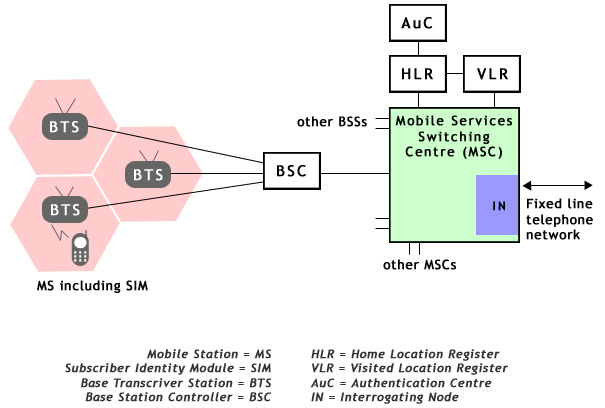
\includegraphics[scale=0.7]{gsmNetworkComponents}
\caption[GSM network components]{GSM network components.
\emph{Source: \url{http://wireless.arcada.fi/MOBWI/material/CN\_1\_2.html}}}
\end{figure}




\subsection{Network and Switching Subsystem (NSS)}

The NSS is made up of an MSC and a Visitor Location Register (VLR). An MSC 
\begin{itemize} 
\item sets up, controls and shuts down connections
\item handles call charges
\item manages additionals services like call forwarding, call blocking, etc.
\end{itemize}

A VLR contains all the subscriber data of the phones being served by the accompanying MSC. It contains their location data too. The VLR also maintains data about the SIMs that do not belong to the network but have roamed into the network. The area served by an MSC is called a MSC/VLR service area.

\begin{figure}
\centering
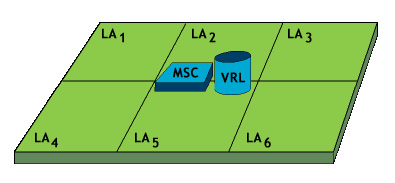
\includegraphics[scale=0.7]{mscvlrServiceArea}
\caption[MSC/VLR Service Area]{MSC/VLR Service Area.
\emph{Source: \url{http://wireless.arcada.fi/MOBWI/material/CN\_1\_2.html}}}
\end{figure}

\subsection{The Operation Subsystem (OSS)}

The OSS consists of :
\begin{itemize}
\item the Operation and Maintenance Center (OMC)
\item the Authentication Center (AuC)
\item the Home Location Register (HLR)
\item the Equipment Identity Register (EIR)
\end{itemize}

The OSS is responsible for
\begin{itemize}
\item network management functions like service provisioning, network configuration, fault management, etc.
\item billing calls
\item administering subscribers
\end{itemize}

The AuC controls all the encryption algorithms used for verifying the SIMs. The EIR contains the serial numbers of all the MSs (mobile phones) being served. The HLR contains the subscriber data and location data of all the SIMs in different parts of the network.

\subsection{GSM Network Areas}

The area covered by a GSM operator is called a PLMN Service Area. A PLMN service area is made up of several MSC/VLR service areas. The hierarchy of service areas is as follows:
\begin{itemize}
\item PLMN service area,
\item MSC/VLR service area,
\item Location Area and
\item Network Cell
\end{itemize}
\begin{figure}
\centering
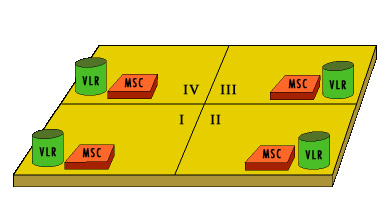
\includegraphics[scale=0.7]{PLMNServiceArea}
\caption[A PLMN Service Area for a GSM operator]{A PLMN Service Area for a GSM operator.
\emph{Source: \url{http://wireless.arcada.fi/MOBWI/material/CN\_1\_2.html}}}
\end{figure}



\section{Protocol Architecture}
The data communication protocols in a GSM network are implemented to work over the bearer\footnote{A bearer data channel is a channel that carries call content i.e.
one that does not carry signaling.} data channel. 
The GSM protocol architecture is structured into three independent planes:
\begin{itemize}
 \item user plane
 \item control plane
 \item management plane
\end{itemize}
\begin{figure}
\centering
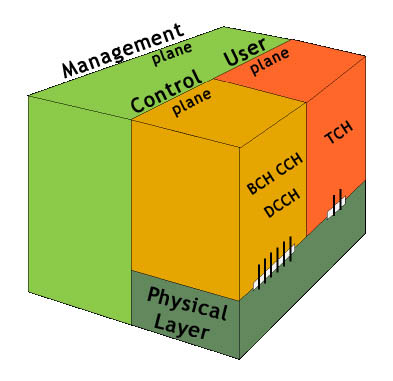
\includegraphics[scale=0.7]{gsmPlanes}
\caption[GSM protocol architecture planes]{GSM protocol architecture planes.
\emph{Source: \url{http://wireless.arcada.fi/MOBWI/material/CN\_1\_3.html}}}
\end{figure}

The user plane defines protocols for handling the voice and user data. 
At the Um interface, the traffic control channel (TCH) is used to carry the user data.


The control plane defines protocols for controlling connections by using signalling data.
The signalling data are carried over logical channels called Dm-channels (wireless analog of the D-channels for wired interface).
The spare capacities of the Dm-channels are used for carrying user data.
Eventually all logical channels have to multiplexed onto the physical channel.


The management plane takes care of the coordination between different planes.
It also manages functions related to the control and/or user planes.
The management plane handles things like network configuration, network fault, etc.

\begin{figure}
\centering
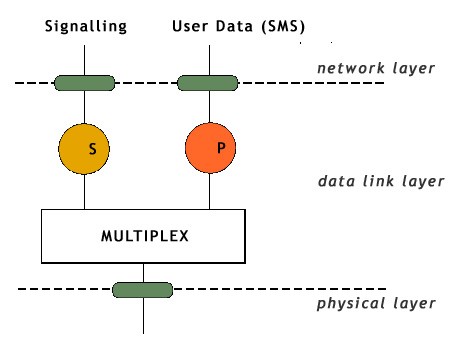
\includegraphics[scale=0.7]{logicalChannelsUserControl}
\caption[Logical channels for user plane data and control plane signalling]{Logical channels for user plane data and control plane signalling.
\emph{Source: \url{http://wireless.arcada.fi/MOBWI/material/CN\_1\_3.html}}}
\end{figure}

\subsection{Signalling Transmission}
In GSM, the network nodes exchange signaling information with each other to establish, control and terminate connections.
The various interfaces in a GSM network are:
\begin{itemize}
 \item MS-BTS: Um
 \item BTS-BSC: Abis
 \item BSC-MSC: A
 \item MSC-VLR: B
 \item MSC-HLR: C
 \item VLR-HLR: D
 \item MSC-MSC: E
 \item MSC-EIR: F
 \item VLR-VLR: G
\end{itemize}

The Um interface is the only interface that uses the wireless physical medium for carrying signals. The rest of the interfaces all use wired and digital mediums.

\subsubsection{\uppercase{Data Link Layer (Layer 2) protocols}}

\begin{description}
 \item [Link Access Protocol, Dm-channel (LAPDm)] is a layer 2 protocol that provides safe, reliable connections to layer 3 protocols. It is a wireless-adapted version of 
 the standard Link Access Protocol, D-channel (LAPD) of ISDN. It works in two modes: Unacknowledged and Acknowledged. In Unacknowledged mode it operates without acknowledgement,
 without error correction and without flow control. While in acknowledged mode, it asserts acknowledgement, error correction is done by resending and flow is controlled.
 \item [Message Transfer Part (MTP)] is the standard ISDN message transport part of Signaling System 7 (SS7). The networking layers covered by MTP cannot be mapped
 one-to-one to the OSI model\footnote{Operation Systems Interconnection model}. But it covers layer 1, layer 2 and parts of layer 3 from the OSI model. The parts of layer 3
 not covered by MTP are covered by Signalling Connection Control Part (SCCP).
\end{description}


